% Seminar 2 - Page 2 (continued from Page 1, 10-Oct-1994).
% Fragment for % Seminar 2 - Page 2 (continued from Page 1, 10-Oct-1994).
% Fragment for % Seminar 2 - Page 2 (continued from Page 1, 10-Oct-1994).
% Fragment for % Seminar 2 - Page 2 (continued from Page 1, 10-Oct-1994).
% Fragment for \input{seminars/pages/seminar2-pagina2-en}; no preamble.
% EDITORIAL NOTES:
% - The sketch of A, B, Im f, and the return arrow r has been redrawn
%   schematically in TikZ, not reconstructed geometrically point for point.
% - In the definition of r, the preimage symbol is provisionally read as u.
% - An abbreviated phrase after "Let f:A -> B" in Exercise 3 is illegible;
%   it has not been expanded speculatively.
% - Selecting a preimage for each y in B to construct s generally invokes
%   the axiom of choice; this assumption is not mentioned in the manuscript.
% - The epimorphism condition is depicted by parallel arrows; the source
%   page does not provide a proof of the full equivalence.

\subsection*{Seminar 2 - Page 2}

\noindent\fbox{$a\Rightarrow b$}\quad
\[
\begin{tikzcd}[column sep=large,row sep=small]
A \arrow[r,"f"] & B \arrow[d,"r"]\\
 & A
\end{tikzcd}
\qquad r(f(u))=u.
\]

% The manuscript sketches the sets A and B, the image of f in B,
% and a return arrow r: B -> A.
\begin{center}
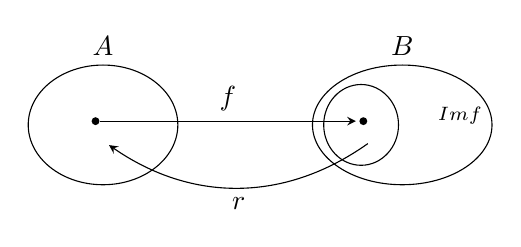
\begin{tikzpicture}[>=stealth,scale=.95]
  \draw (-2,0) ellipse (1.0 and .8);
  \draw (2,0) ellipse (1.2 and .8);
  \node at (-2,1.05) {$A$};
  \node at (2,1.05) {$B$};
  \draw (1.45,0) ellipse (.50 and .54);
  \node[font=\scriptsize] at (2.77,.13) {$\operatorname{Im}f$};
  \fill (-2.1,.05) circle (1.5pt);
  \fill (1.48,.05) circle (1.5pt);
  \draw[->] (-2.04,.05) -- (1.38,.05) node[midway,above] {$f$};
  \draw[->] (1.54,-.25) to[bend left=35] node[below] {$r$} (-1.92,-.27);
\end{tikzpicture}
\end{center}

\noindent Let $a\in A$; define
\[
r(y)=
\begin{cases}
u, & \text{if }f(u)=y,\\
a, & \text{if }y\notin\operatorname{Im}f.
\end{cases}
\]
\noindent Since $f$ is injective, $r$ is well-defined.
\[
(r\circ f)(u)=r(f(u))=u
\quad\Longrightarrow\quad r\circ f=1_A.
\]

\medskip
\noindent\fbox{$b\Rightarrow a$}\quad
Let $f(x_1)=f(x_2)$. Then
\[
r(f(x_1))=r(f(x_2))
\quad\Longrightarrow\quad x_1=x_2
\quad\Longrightarrow\quad f\text{ injective}.
\]

\medskip
\noindent\fbox{3}\quad Let $f:A\longrightarrow B$.
\begin{enumerate}
\item[a)] $f$ is surjective.
\item[b)] $f$ has a section (there exists $s:B\longrightarrow A$ such that $f\circ s=1_B$).
\item[c)] $f$ is an epimorphism:
\[
\begin{tikzcd}[column sep=large]
A \arrow[r,"f"] & B
\arrow[r,shift left=.55ex,"f_1"]
\arrow[r,shift right=.55ex,"f_2"'] & X
\end{tikzcd}
\]
\end{enumerate}

\noindent\underline{Solution}

\noindent $a)\Rightarrow b)$.
\noindent $(\forall)\,y\in B$, $(\exists)\,x\in A$ such that $y=f(x)$.
\[
f^{-1}(y)=\{x\in A\mid f(x)=y\}\neq\varnothing.
\]
\noindent For every $y\in B$, choose $x_B\in f^{-1}(y)$, and put
\[
s(y)=x_B,\qquad (f\circ s)(y)=f(x_B)=y.
\]

\medskip
\noindent $b)\Rightarrow a)$.
\[
f\circ s\text{ surjective}\quad\Longrightarrow\quad f\text{ surjective}.
\]
; no preamble.
% EDITORIAL NOTES:
% - The sketch of A, B, Im f, and the return arrow r has been redrawn
%   schematically in TikZ, not reconstructed geometrically point for point.
% - In the definition of r, the preimage symbol is provisionally read as u.
% - An abbreviated phrase after "Let f:A -> B" in Exercise 3 is illegible;
%   it has not been expanded speculatively.
% - Selecting a preimage for each y in B to construct s generally invokes
%   the axiom of choice; this assumption is not mentioned in the manuscript.
% - The epimorphism condition is depicted by parallel arrows; the source
%   page does not provide a proof of the full equivalence.

\subsection*{Seminar 2 - Page 2}

\noindent\fbox{$a\Rightarrow b$}\quad
\[
\begin{tikzcd}[column sep=large,row sep=small]
A \arrow[r,"f"] & B \arrow[d,"r"]\\
 & A
\end{tikzcd}
\qquad r(f(u))=u.
\]

% The manuscript sketches the sets A and B, the image of f in B,
% and a return arrow r: B -> A.
\begin{center}
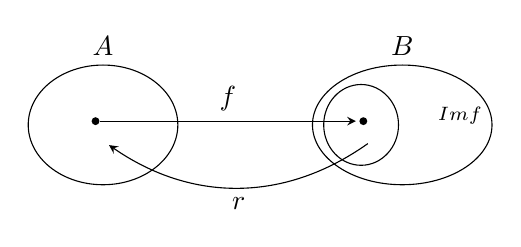
\begin{tikzpicture}[>=stealth,scale=.95]
  \draw (-2,0) ellipse (1.0 and .8);
  \draw (2,0) ellipse (1.2 and .8);
  \node at (-2,1.05) {$A$};
  \node at (2,1.05) {$B$};
  \draw (1.45,0) ellipse (.50 and .54);
  \node[font=\scriptsize] at (2.77,.13) {$\operatorname{Im}f$};
  \fill (-2.1,.05) circle (1.5pt);
  \fill (1.48,.05) circle (1.5pt);
  \draw[->] (-2.04,.05) -- (1.38,.05) node[midway,above] {$f$};
  \draw[->] (1.54,-.25) to[bend left=35] node[below] {$r$} (-1.92,-.27);
\end{tikzpicture}
\end{center}

\noindent Let $a\in A$; define
\[
r(y)=
\begin{cases}
u, & \text{if }f(u)=y,\\
a, & \text{if }y\notin\operatorname{Im}f.
\end{cases}
\]
\noindent Since $f$ is injective, $r$ is well-defined.
\[
(r\circ f)(u)=r(f(u))=u
\quad\Longrightarrow\quad r\circ f=1_A.
\]

\medskip
\noindent\fbox{$b\Rightarrow a$}\quad
Let $f(x_1)=f(x_2)$. Then
\[
r(f(x_1))=r(f(x_2))
\quad\Longrightarrow\quad x_1=x_2
\quad\Longrightarrow\quad f\text{ injective}.
\]

\medskip
\noindent\fbox{3}\quad Let $f:A\longrightarrow B$.
\begin{enumerate}
\item[a)] $f$ is surjective.
\item[b)] $f$ has a section (there exists $s:B\longrightarrow A$ such that $f\circ s=1_B$).
\item[c)] $f$ is an epimorphism:
\[
\begin{tikzcd}[column sep=large]
A \arrow[r,"f"] & B
\arrow[r,shift left=.55ex,"f_1"]
\arrow[r,shift right=.55ex,"f_2"'] & X
\end{tikzcd}
\]
\end{enumerate}

\noindent\underline{Solution}

\noindent $a)\Rightarrow b)$.
\noindent $(\forall)\,y\in B$, $(\exists)\,x\in A$ such that $y=f(x)$.
\[
f^{-1}(y)=\{x\in A\mid f(x)=y\}\neq\varnothing.
\]
\noindent For every $y\in B$, choose $x_B\in f^{-1}(y)$, and put
\[
s(y)=x_B,\qquad (f\circ s)(y)=f(x_B)=y.
\]

\medskip
\noindent $b)\Rightarrow a)$.
\[
f\circ s\text{ surjective}\quad\Longrightarrow\quad f\text{ surjective}.
\]
; no preamble.
% EDITORIAL NOTES:
% - The sketch of A, B, Im f, and the return arrow r has been redrawn
%   schematically in TikZ, not reconstructed geometrically point for point.
% - In the definition of r, the preimage symbol is provisionally read as u.
% - An abbreviated phrase after "Let f:A -> B" in Exercise 3 is illegible;
%   it has not been expanded speculatively.
% - Selecting a preimage for each y in B to construct s generally invokes
%   the axiom of choice; this assumption is not mentioned in the manuscript.
% - The epimorphism condition is depicted by parallel arrows; the source
%   page does not provide a proof of the full equivalence.

\subsection*{Seminar 2 - Page 2}

\noindent\fbox{$a\Rightarrow b$}\quad
\[
\begin{tikzcd}[column sep=large,row sep=small]
A \arrow[r,"f"] & B \arrow[d,"r"]\\
 & A
\end{tikzcd}
\qquad r(f(u))=u.
\]

% The manuscript sketches the sets A and B, the image of f in B,
% and a return arrow r: B -> A.
\begin{center}
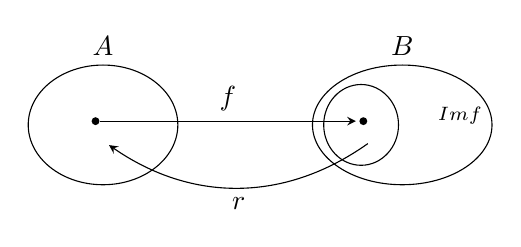
\begin{tikzpicture}[>=stealth,scale=.95]
  \draw (-2,0) ellipse (1.0 and .8);
  \draw (2,0) ellipse (1.2 and .8);
  \node at (-2,1.05) {$A$};
  \node at (2,1.05) {$B$};
  \draw (1.45,0) ellipse (.50 and .54);
  \node[font=\scriptsize] at (2.77,.13) {$\operatorname{Im}f$};
  \fill (-2.1,.05) circle (1.5pt);
  \fill (1.48,.05) circle (1.5pt);
  \draw[->] (-2.04,.05) -- (1.38,.05) node[midway,above] {$f$};
  \draw[->] (1.54,-.25) to[bend left=35] node[below] {$r$} (-1.92,-.27);
\end{tikzpicture}
\end{center}

\noindent Let $a\in A$; define
\[
r(y)=
\begin{cases}
u, & \text{if }f(u)=y,\\
a, & \text{if }y\notin\operatorname{Im}f.
\end{cases}
\]
\noindent Since $f$ is injective, $r$ is well-defined.
\[
(r\circ f)(u)=r(f(u))=u
\quad\Longrightarrow\quad r\circ f=1_A.
\]

\medskip
\noindent\fbox{$b\Rightarrow a$}\quad
Let $f(x_1)=f(x_2)$. Then
\[
r(f(x_1))=r(f(x_2))
\quad\Longrightarrow\quad x_1=x_2
\quad\Longrightarrow\quad f\text{ injective}.
\]

\medskip
\noindent\fbox{3}\quad Let $f:A\longrightarrow B$.
\begin{enumerate}
\item[a)] $f$ is surjective.
\item[b)] $f$ has a section (there exists $s:B\longrightarrow A$ such that $f\circ s=1_B$).
\item[c)] $f$ is an epimorphism:
\[
\begin{tikzcd}[column sep=large]
A \arrow[r,"f"] & B
\arrow[r,shift left=.55ex,"f_1"]
\arrow[r,shift right=.55ex,"f_2"'] & X
\end{tikzcd}
\]
\end{enumerate}

\noindent\underline{Solution}

\noindent $a)\Rightarrow b)$.
\noindent $(\forall)\,y\in B$, $(\exists)\,x\in A$ such that $y=f(x)$.
\[
f^{-1}(y)=\{x\in A\mid f(x)=y\}\neq\varnothing.
\]
\noindent For every $y\in B$, choose $x_B\in f^{-1}(y)$, and put
\[
s(y)=x_B,\qquad (f\circ s)(y)=f(x_B)=y.
\]

\medskip
\noindent $b)\Rightarrow a)$.
\[
f\circ s\text{ surjective}\quad\Longrightarrow\quad f\text{ surjective}.
\]
; no preamble.
% EDITORIAL NOTES:
% - The sketch of A, B, Im f, and the return arrow r has been redrawn
%   schematically in TikZ, not reconstructed geometrically point for point.
% - In the definition of r, the preimage symbol is provisionally read as u.
% - An abbreviated phrase after "Let f:A -> B" in Exercise 3 is illegible;
%   it has not been expanded speculatively.
% - Selecting a preimage for each y in B to construct s generally invokes
%   the axiom of choice; this assumption is not mentioned in the manuscript.
% - The epimorphism condition is depicted by parallel arrows; the source
%   page does not provide a proof of the full equivalence.

\subsection*{Seminar 2 - Page 2}

\noindent\fbox{$a\Rightarrow b$}\quad
\[
\begin{tikzcd}[column sep=large,row sep=small]
A \arrow[r,"f"] & B \arrow[d,"r"]\\
 & A
\end{tikzcd}
\qquad r(f(u))=u.
\]

% The manuscript sketches the sets A and B, the image of f in B,
% and a return arrow r: B -> A.
\begin{center}
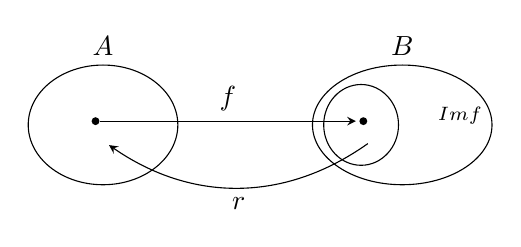
\begin{tikzpicture}[>=stealth,scale=.95]
  \draw (-2,0) ellipse (1.0 and .8);
  \draw (2,0) ellipse (1.2 and .8);
  \node at (-2,1.05) {$A$};
  \node at (2,1.05) {$B$};
  \draw (1.45,0) ellipse (.50 and .54);
  \node[font=\scriptsize] at (2.77,.13) {$\operatorname{Im}f$};
  \fill (-2.1,.05) circle (1.5pt);
  \fill (1.48,.05) circle (1.5pt);
  \draw[->] (-2.04,.05) -- (1.38,.05) node[midway,above] {$f$};
  \draw[->] (1.54,-.25) to[bend left=35] node[below] {$r$} (-1.92,-.27);
\end{tikzpicture}
\end{center}

\noindent Let $a\in A$; define
\[
r(y)=
\begin{cases}
u, & \text{if }f(u)=y,\\
a, & \text{if }y\notin\operatorname{Im}f.
\end{cases}
\]
\noindent Since $f$ is injective, $r$ is well-defined.
\[
(r\circ f)(u)=r(f(u))=u
\quad\Longrightarrow\quad r\circ f=1_A.
\]

\medskip
\noindent\fbox{$b\Rightarrow a$}\quad
Let $f(x_1)=f(x_2)$. Then
\[
r(f(x_1))=r(f(x_2))
\quad\Longrightarrow\quad x_1=x_2
\quad\Longrightarrow\quad f\text{ injective}.
\]

\medskip
\noindent\fbox{3}\quad Let $f:A\longrightarrow B$.
\begin{enumerate}
\item[a)] $f$ is surjective.
\item[b)] $f$ has a section (there exists $s:B\longrightarrow A$ such that $f\circ s=1_B$).
\item[c)] $f$ is an epimorphism:
\[
\begin{tikzcd}[column sep=large]
A \arrow[r,"f"] & B
\arrow[r,shift left=.55ex,"f_1"]
\arrow[r,shift right=.55ex,"f_2"'] & X
\end{tikzcd}
\]
\end{enumerate}

\noindent\underline{Solution}

\noindent $a)\Rightarrow b)$.
\noindent $(\forall)\,y\in B$, $(\exists)\,x\in A$ such that $y=f(x)$.
\[
f^{-1}(y)=\{x\in A\mid f(x)=y\}\neq\varnothing.
\]
\noindent For every $y\in B$, choose $x_B\in f^{-1}(y)$, and put
\[
s(y)=x_B,\qquad (f\circ s)(y)=f(x_B)=y.
\]

\medskip
\noindent $b)\Rightarrow a)$.
\[
f\circ s\text{ surjective}\quad\Longrightarrow\quad f\text{ surjective}.
\]
